\subsection{Architecture}

The platform's architecture is shown in Figure~\ref{platform_architecture_ref}.

\begin{figure}[h!]
    \begin{center}
        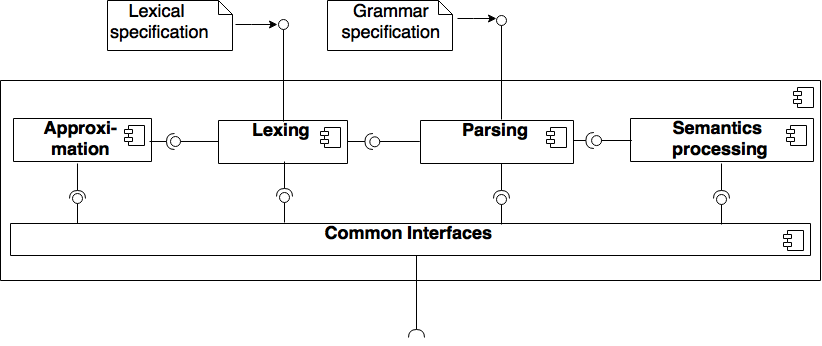
\includegraphics[scale=0.3]{Figures/SELYCcomponents.png}
    \end{center}
    \caption{The platform's architecture}
    \label{platform_architecture_ref}
\end{figure} 

The Approximation component is responsible for building the set of strings with embedded code that can be produced by the host language program. The elements of that set are to be statically analysed. This set can be considered as a language where the words are the strings with embedded code. In general the language can be recursively enumerable. Many problems are undecidable for this class of languages that makes it hard to work with. One possible solution is to build an upper regular approximation of the language we have. In other words we build the regular language that contains all the words of the language we have and, possibly, some other words. It is important to note that the regular language must be as close as possible to the language it approximates. It means the language must keep the number of "extra" words to a minimum. Despite the fact we end up with the approximation of the initial set, working with a regular language makes the further analysis much easier. Moreover, regular languages can always be represented as FSA that is convenient to manipulate.

The Approximation component accepts a generalized CFG with some additional information as an input. As an output it produces the FSA that encodes the approximated set of strings with embedded code.

The lexing component consist of two parts. The first one is the lexer's generator which generates finite-state transducer(FST,~~\cite{FST:ref}) from the provided lexical specification of the string-embedded-language. The second one is the interpreter which analyzes the data structure passed using generated FST. The lexing component accepts FSA over symbols alphabet and produces the FSA over alphabet of processed language tokens.

The parser generator is based on the RNGLR algorithm~\cite{RNGLR:ref}. Using the grammar of the language processed the generator builds parse tables. Then the analyzer, which is implemented as a separate library, parses the FSA that was obtained after the lexical analysis. The result is a shared packed parse forest (SPPF~\cite{SPPF:ref}) which is a compact structure that allows to reuse common nodes along different ASTs. This structure can be used for the further processing: for additional information extraction or to implement such IDE functionality as "go to definition".